% A rectangular contour gamma subdivided into four sub-rectangles
% gamma_a, gamma_b, gamma_c, gamma_d; the inner edges cancel in pairs.
% (Drawn with a margin for clarity; in reality the inner edges overlap.)
% Source: book/tex/complex-ana/holomorphic.tex
%   (section: Optional: Proof that holomorphic functions are analytic).
\documentclass[border=2mm]{standalone}
\usepackage{tikz}
\usetikzlibrary{arrows.meta, decorations.markings}
\begin{document}
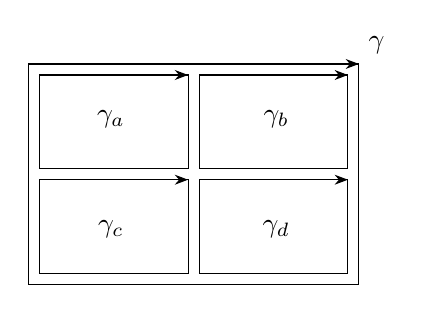
\begin{tikzpicture}[scale=0.7,
    decoration={markings, mark=at position 0.5 with {\arrow{Stealth}}}]
  \tikzset{rr/.style={postaction={decorate}}}
  \draw[rr] (0,0) rectangle (6,4);
  \draw[rr] (0.2,0.2) rectangle (2.9,1.9);
  \draw[rr] (3.1,0.2) rectangle (5.8,1.9);
  \draw[rr] (0.2,2.1) rectangle (2.9,3.8);
  \draw[rr] (3.1,2.1) rectangle (5.8,3.8);
  \node at (6,4) [above right] {$\gamma$};
  \node at (1.5,3) {$\gamma_a$};
  \node at (4.5,3) {$\gamma_b$};
  \node at (1.5,1) {$\gamma_c$};
  \node at (4.5,1) {$\gamma_d$};
\end{tikzpicture}
\end{document}
